\section{Risultati finali}
In conclusione, dopo il completamento del componente \textit{frontend}, abbiamo pubblicato il prototipo 
su \textbf{Artifactory}, un repository, interno all'azienda,  di librerie e componenti software, per poterlo utilizzare
in un progetto di prova.\\
Il prototipo poi è stato incluso in alcuni progetti di prova, per testare la sua funzionalità e la sua integrazione
con il resto del sistema.\\
Per includerlo in un progetto, è necessario innanzitutto aggiungere il frammento di codice \ref{lst:settings.gradle} al file \textit{settings.gradle} del progetto,
in modo da poter scaricare le dipendenze dal repository di Artifactory.\\
\begin{lstlisting}[language=Groovy, 
  caption=Configurazione per includere la dipendenza del \textit{plugin} in un progetto,
  label=lst:settings.gradle
  ]
  buildscript {

    repositories {
        maven {
            url "${artifactory_contextUrl}/${artifactory_repo}"
            credentials {
                username = "${artifactory_user}"
                password = "${artifactory_password}"
            }
        }
    }
    dependencies {
        classpath("com.smi:smi-dependency-analyzer:1.0.0-SNAPSHOT-1")
    }
}
\end{lstlisting}

Successivamente, è necessario aggiungere il frammento di codice \ref{lst:build.gradle} al file \textit{build.gradle} del progetto,
in modo da applicare il plugin.\\

\begin{lstlisting}[language=Groovy, 
  caption=Configurazione per applicare il \textit{plugin} in un progetto,
  label=lst:build.gradle
  ]
  apply plugin: 'com.smi.SmiDependencyAnalyzer'

  smi_dependency_analyzer {
    username = "deployer"
    password = "PASSWORD"
    url = "http://localhost:8080/smi-dependency-store"

    npmProject {
        packageJson = "/Users/smi/app/client/package.json"
        packageLockJson = "/Users/smi/app/client/package-lock.json"
    }
}

\end{lstlisting}

Infine, sarà sufficiente eseguire il comando \textit{gradle smiDependencyAnalyzer} per avviare il \textit{plugin}.\\
Solo dopo aver eseguito questi passaggi, sarà possibile visualizzare l'albero delle dipendenze del progetto,
attraverso l'interfaccia grafica. \\
Per farlo sarà sufficiente aprire il \textit{browser} e navigare all'indirizzo \url{http://INDIRIZZO_WEB_SERVER/smi-dependency-store}
ed accedere con le credenziali di dominio aziendale, come mostrato nella figura \ref*{fig:login}.\\
Dopo quest'ultima operazione si ha accesso a tutte le funzionalità descritte in precedenza.

\begin{figure}[!h]
  \centering
  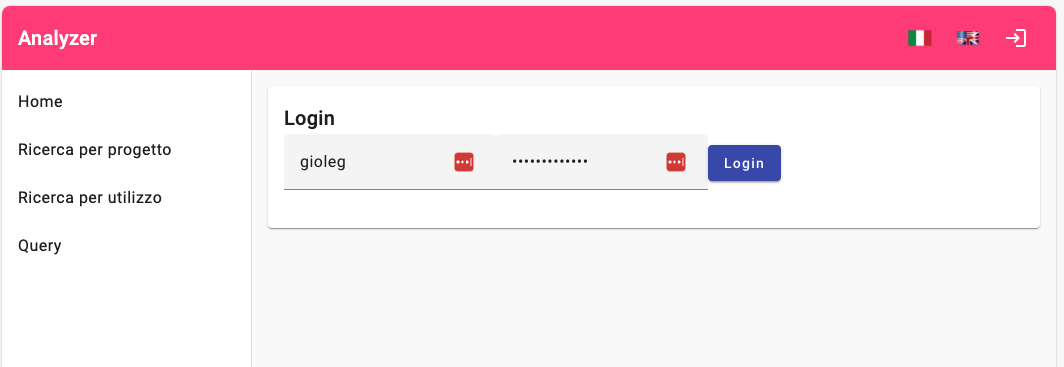
\includegraphics[width=0.8\textwidth]{login}
  \caption{Pagina di login}
  \label{fig:login}
\end{figure}

